%% Figure index for HW-1 paper
%% Auto-generated by generate_all.py

\section{Figures}

\begin{figure}[htbp]
  \centering
  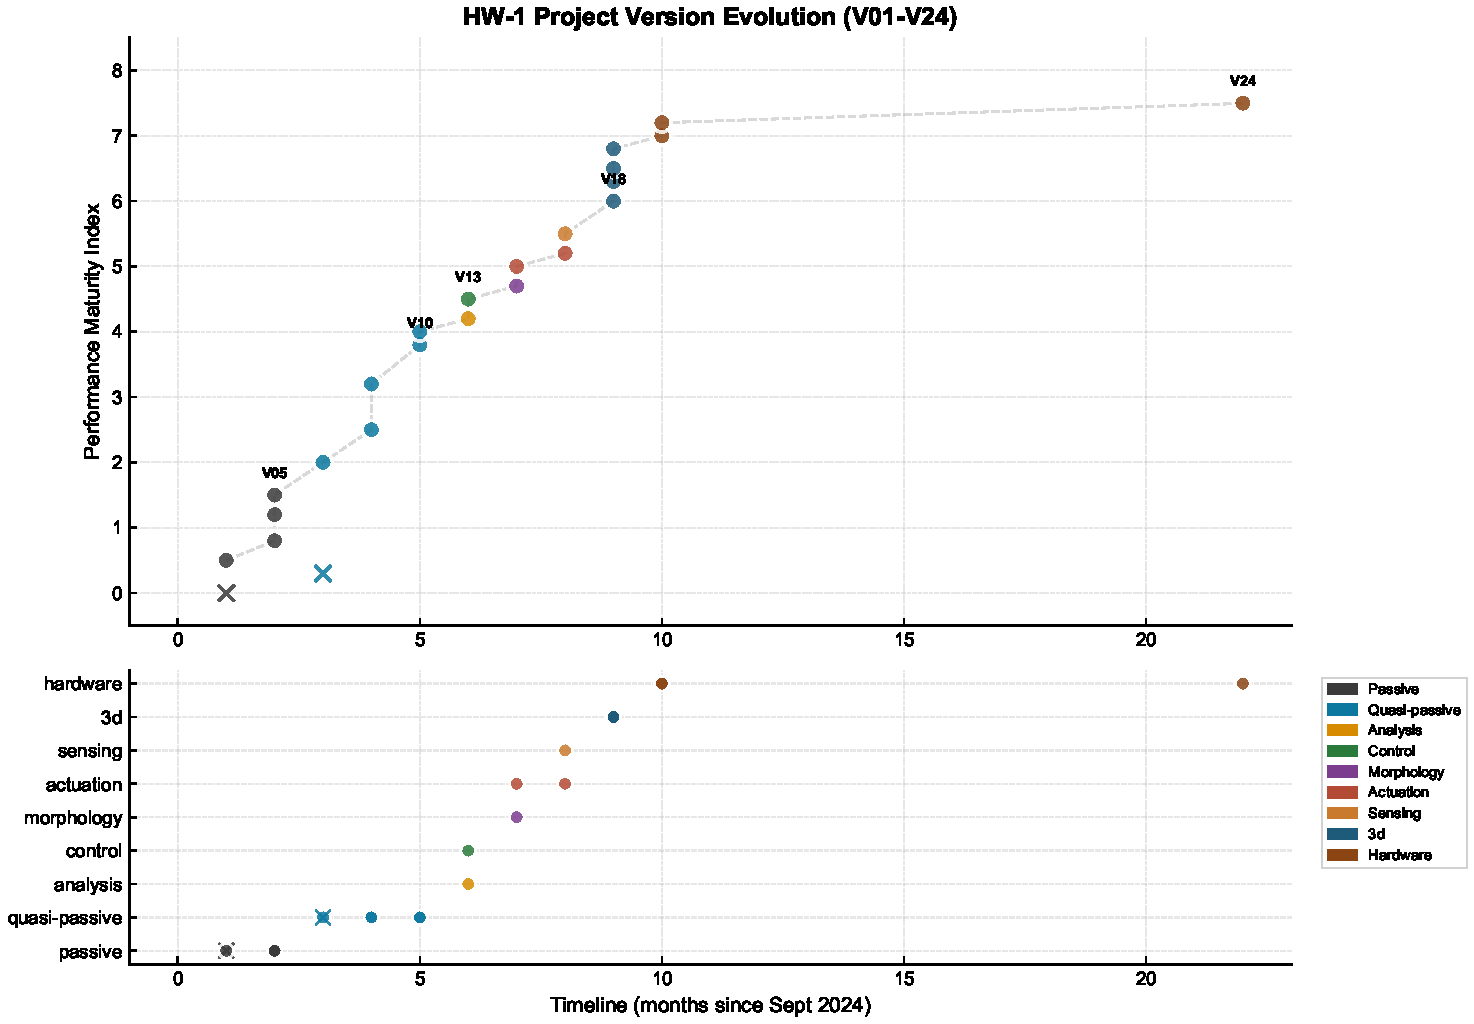
\includegraphics[width=\textwidth]{paper_figures/output/fig1_version_evolution.pdf}
  \caption{Version Evolution Timeline: Development progress from V01 (Compass Gait) to V24 (Sim-to-Real). 
  Top panel shows performance maturity index progression. Bottom panel shows category distribution across versions.
  Key milestones: V05 (passive limit cycle proof), V10 (rolling foot), V13 (FSM control), V18 (3D stability), V24 (hardware deployment).}
  \label{fig:version_evolution}
\end{figure}

\begin{figure}[htbp]
  \centering
  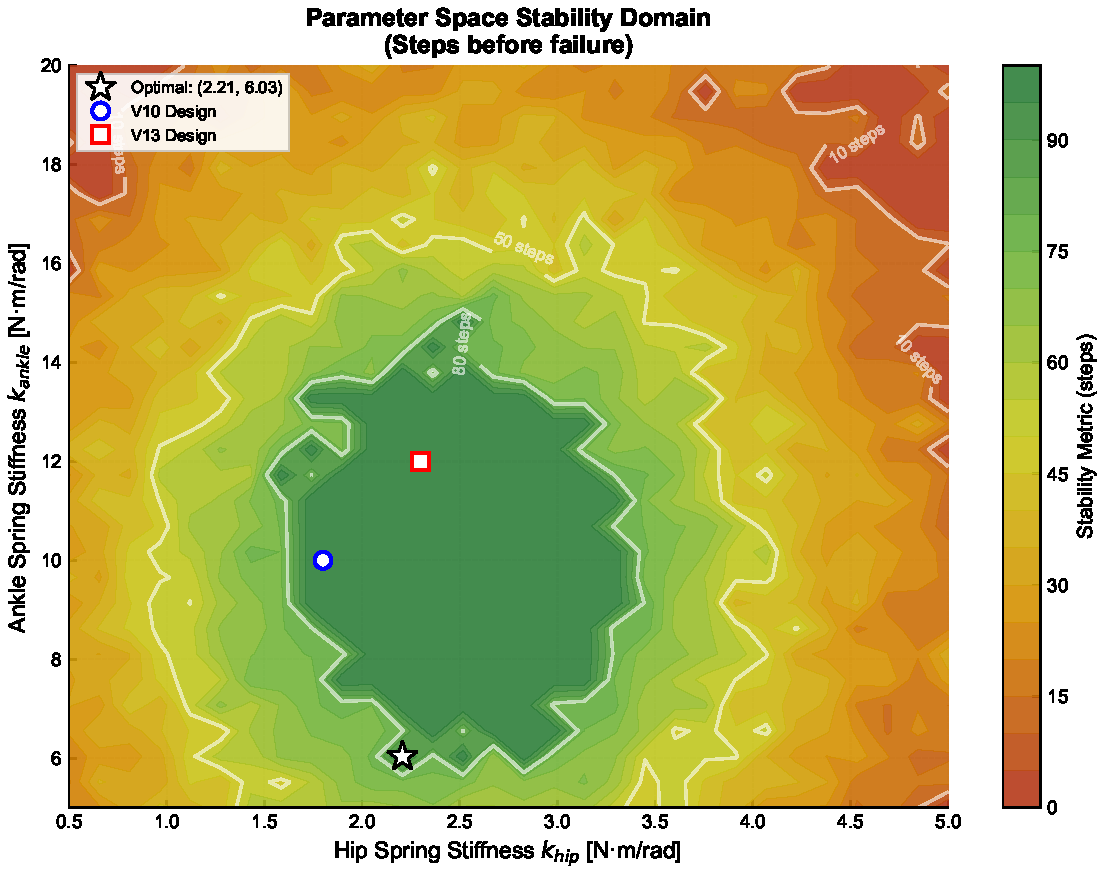
\includegraphics[width=0.85\textwidth]{paper_figures/output/fig2_stability_domain.pdf}
  \caption{Parameter Space Stability Domain: Heatmap showing gait stability (steps before failure) as a function of hip and ankle spring stiffness.
  White star indicates optimal parameters. Blue circle (V10) and red square (V13) show actual design choices.
  Contour lines mark stability thresholds at 10, 50, and 80 steps.}
  \label{fig:stability_domain}
\end{figure}

\begin{figure}[htbp]
  \centering
  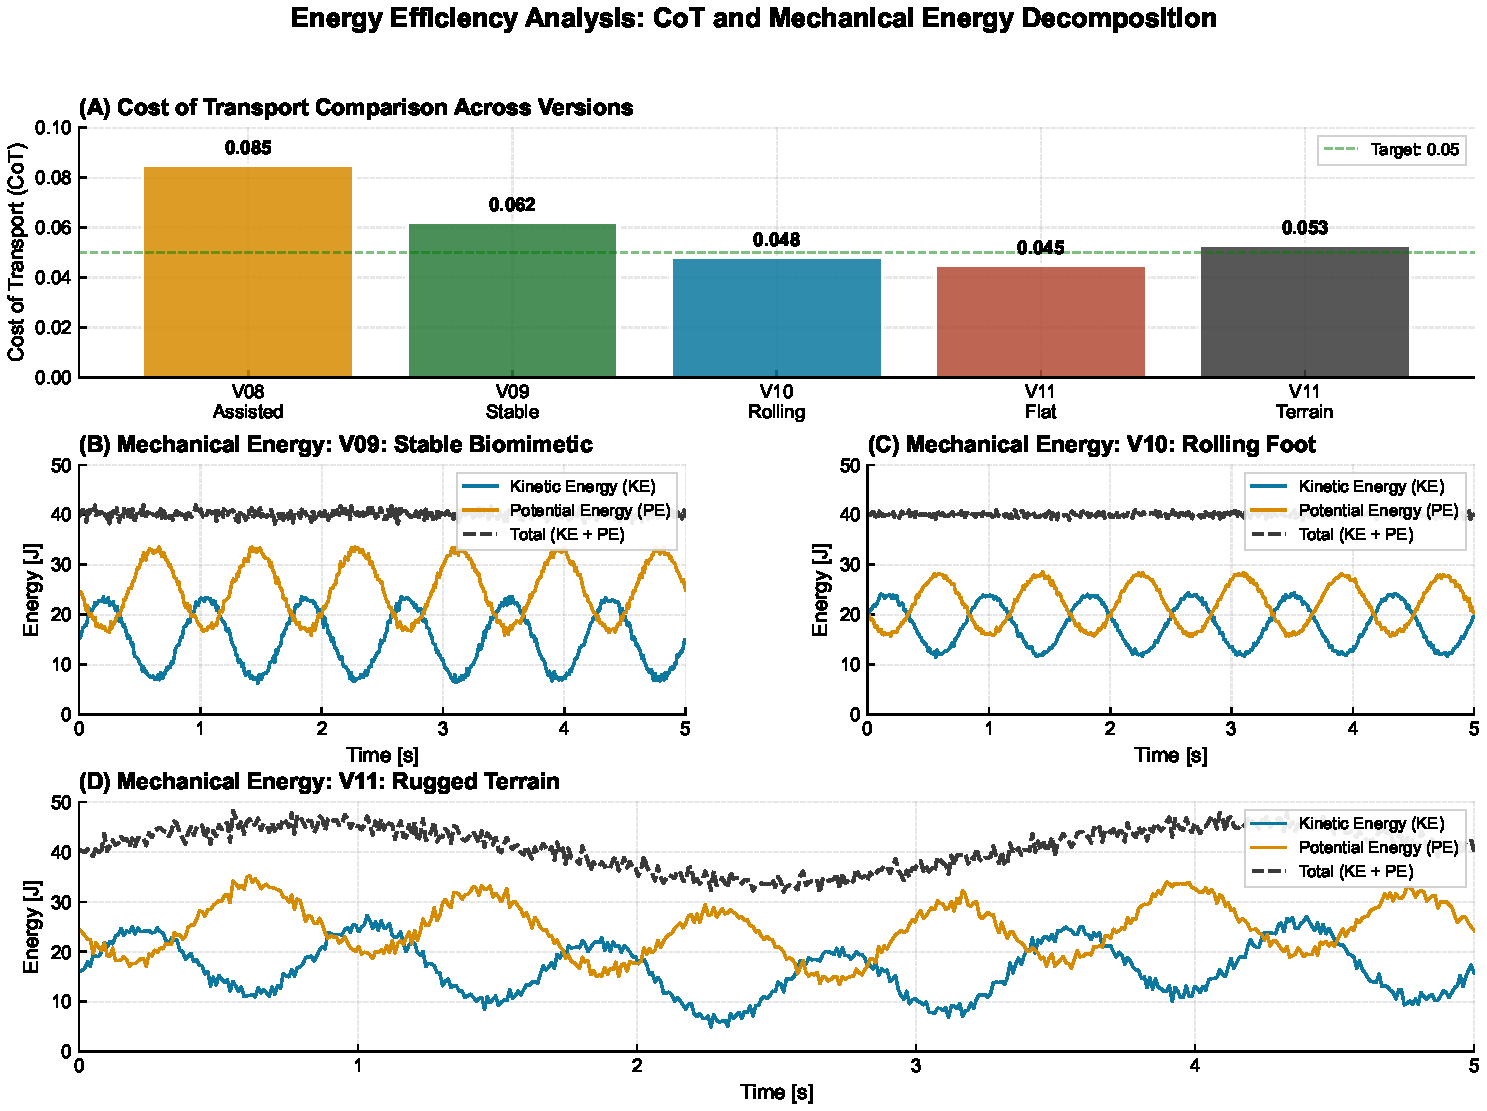
\includegraphics[width=\textwidth]{paper_figures/output/fig3_energy_analysis.pdf}
  \caption{Energy Efficiency Analysis: (A) Cost of Transport comparison across quasi-passive versions.
  V10 achieves lowest CoT of 0.048. (B-D) Mechanical energy decomposition showing kinetic-potential energy exchange
  during periodic gait. V11 terrain case shows larger fluctuations due to ground irregularities.}
  \label{fig:energy_analysis}
\end{figure}

\begin{figure}[htbp]
  \centering
  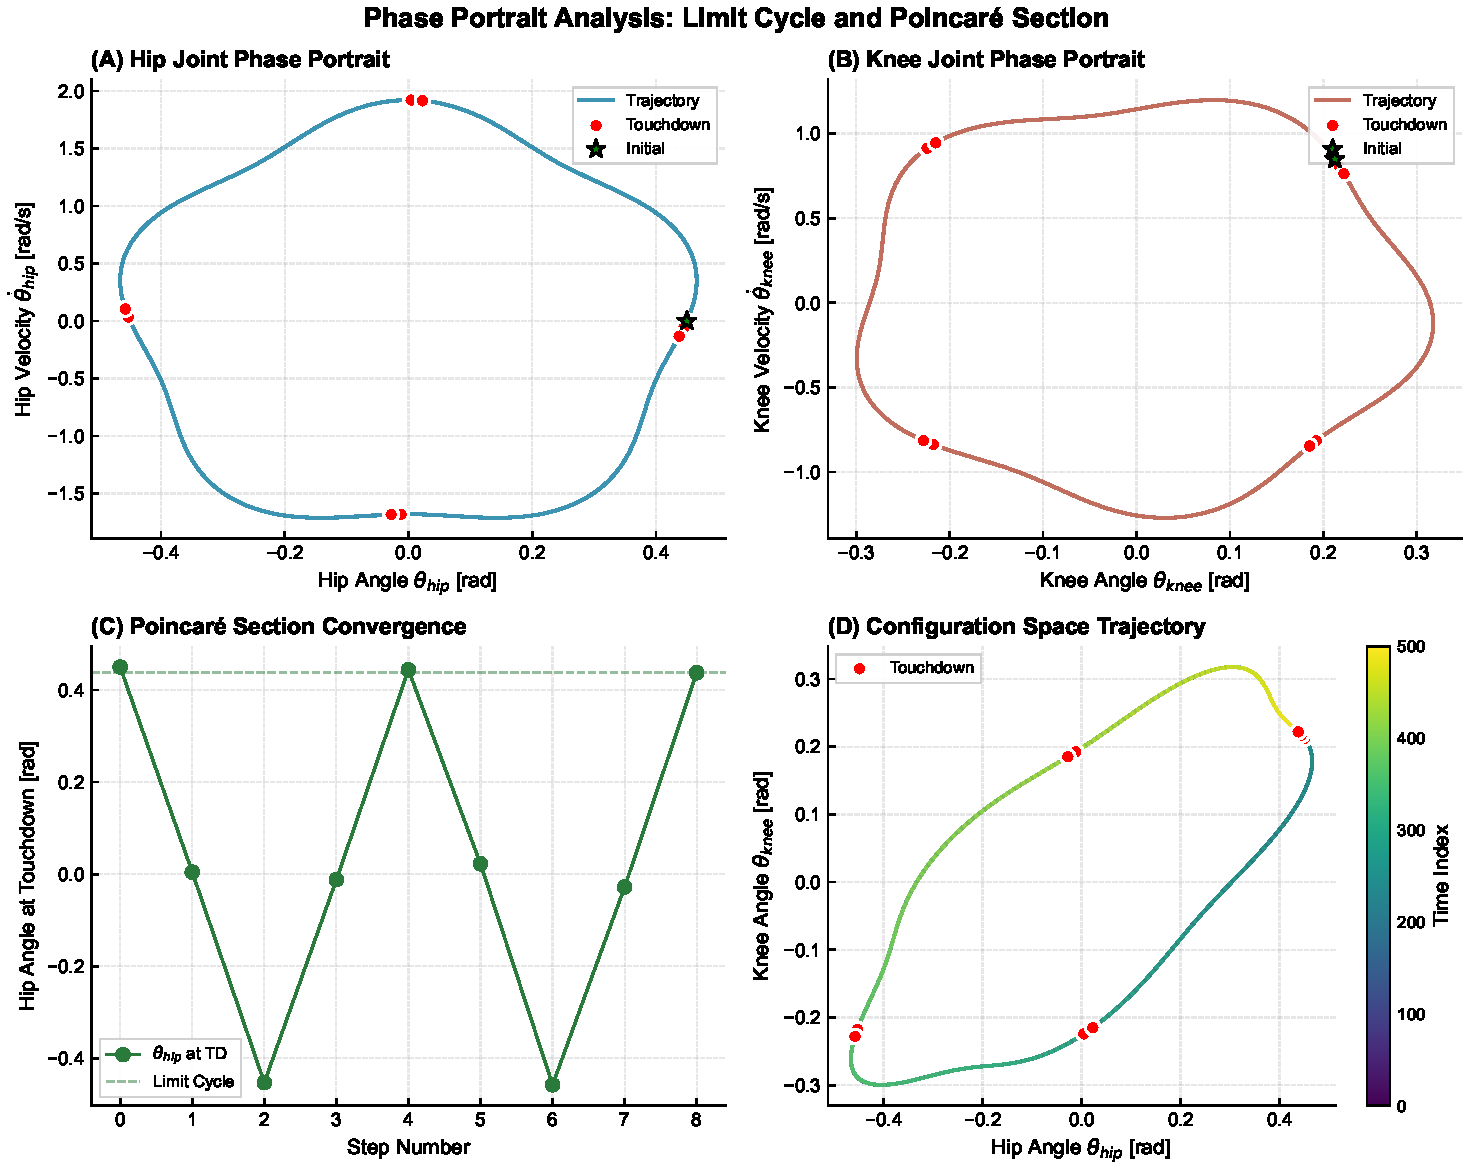
\includegraphics[width=\textwidth]{paper_figures/output/fig4_phase_portrait.pdf}
  \caption{Phase Portrait and Limit Cycle Analysis: (A-B) Hip and knee joint phase space trajectories showing periodic motion.
  Red circles indicate touchdown events (Poincaré section). (C) Convergence to limit cycle demonstrated by consistent touchdown states.
  (D) Configuration space projection colored by time shows coupled hip-knee coordination.}
  \label{fig:phase_portrait}
\end{figure}

\begin{figure}[htbp]
  \centering
  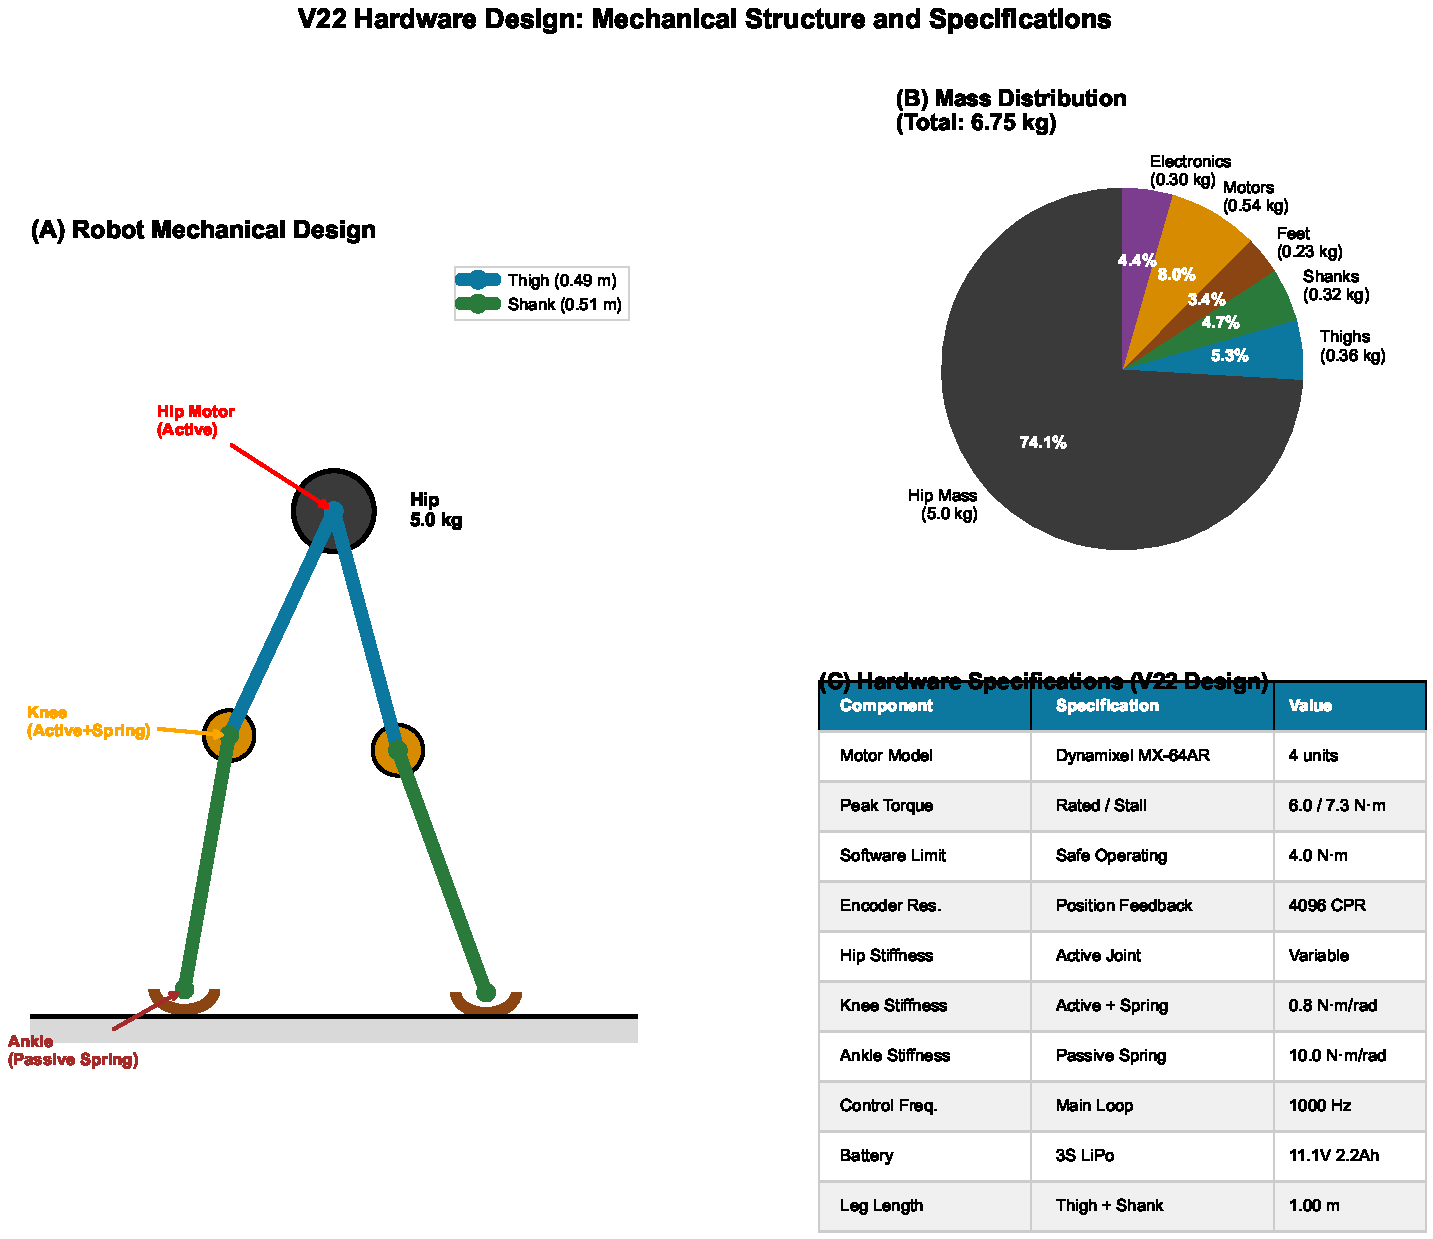
\includegraphics[width=\textwidth]{paper_figures/output/fig5_hardware_specs.pdf}
  \caption{V22 Hardware Design Specifications: (A) Mechanical schematic showing 5-link bipedal structure with total leg length 1.0 m.
  (B) Mass distribution with 74\% concentrated at hip. (C) Actuator and component specifications including
  Dynamixel MX-64AR motors (4 units), spring stiffnesses, and control system parameters.}
  \label{fig:hardware_specs}
\end{figure}

%% Usage in text:
%% Figure~\ref{fig:version_evolution} shows the development timeline...
%% The stability domain (Figure~\ref{fig:stability_domain}) reveals...
%% Energy analysis (Figure~\ref{fig:energy_analysis}) demonstrates...
%% Phase portraits in Figure~\ref{fig:phase_portrait} confirm limit cycle behavior...
%% Hardware specifications (Figure~\ref{fig:hardware_specs}) detail the V22 design...
